\section{Exemplos resolvidos}
\subsubsection*{Exemplo 1}

O exemplo 1 solicita a análise de sobretensões sustentadas e consumo de reativo numa linha de transmissão caracterizada por: $l=150km$, $X^'=0.377\Omega/km;$, $C^'=14nF/km$ e $V_N=500kV$.

Uma vez que a extensão da linha é maior que $80 km$ e menor que $240 km$, o modelo de linha média pode ser aplicado sem maiores problemas. De acordo com a equação matricial \ref{top2:eq:4}, considerando a energização com $I_2=0$, tem-se que a relação entre a tensão de entrada e a de saída será:

\begin{equation} \label{exe:1:1}
    V_1 = \left(\frac{ZY}{2}+1\right)V_2 + ZI_2 = \left(\frac{ZY}{2}+1\right)V_2
\end{equation}

Já o consumo de reativo será: $Q_c = V_1I_1^*$, porém apenas a tensão na entrada é conhecida. Para encontrar a corrente de entrada do quadripolo recorre-se à equação matricial \ref{top2:eq:4}, tomando:

\begin{equation} \label{exe:1:2}
    I_1 = Y\left(\frac{ZY}{4}+1\right)V_2 + \left(\frac{ZY}{2}+1\right)I_2 = Y\left(\frac{ZY}{4}+1\right)V_2
\end{equation}

A sequência do problema é estabelecer os parâmetros longitudinais e transversais da linha e em seguida resolver a sobretensão, assim estabelecendo a tensão ao final do quadripolo. Em seguida esta tensão é utilizada para obter a corrente de entrada do quadripolo, permitindo que, finalmente encontre-se a potência reativa consumida.

Assim, considerando $R=0$, a impedância longitudinal da linha será: $Z = jX^{'}l = j56.55 \Omega$; e a admitância transversal será: $Y = jC^{'} l \times 2\pi f = 791.68 \mu S$. Desta forma os demais valores podem ser obtidos facilmente pelas expressões mostradas anteriormente, assim considerando apenas valores por fase, tem-se uma tensão na saída de $V_2 = 1.0229 p.u$ que corresponde a uma sobretensão de $2.29\%$. No que diz respeito à corrente por fase, já considerando os valores reais, tem-se $I_1 = j231.16 A$ que corresponde a uma potência reativa consumida por fase de $Q_c = 66.72 Mvar$.

\subsubsection*{Exemplo 2}

O exemplo 2 solicita o cálculo da sobretensão e da compensação reativa para $V_1=V_2$ considerando uma linha com os mesmos parâmetros da anterior, porém sendo uma linha longa de $l = 400km$. Desta forma se faz necessário utilizar o modelo de linha longa da equação matricial \ref{top2:eq:5}.

De acordo com a equação do quadripolo, a constante generalizada $A = cosh(\gamma l)$ relaciona a tensão na entrada com a da saída, por meio de $V_1 = A V_1$. Assim, para encontrar o valor de A para a situação atual da linha se faz necessário encontrar $\gamma$ e, consequentemente a densidade de impedância e admitância da linha ($z$ e $y$, respectivamente).

Como $z = jX^{'} = j377 \mu \Omega/m$ e $y = jC^{'} \times 2\pi f = j5.2779 nS/m$ , tem-se que $\gamma = \sqrt{zy} = j1.41 \mu rad/m$. Isso conclui que $A = 0.845$. Esse valor garante uma sobretensão de $18.34\%$  ($1-A^{-1}$). 

Para o projeto do reator de compensação deve ser levada em consideração a equação \ref{top2:eq:comp} que introduz o quadripolo do reator ao quadripolo da linha longa, assim permitindo que a constante generalizada A seja rescrita como: $A^{'}=A+\frac{B}{sL_r}$, onde $L_r$ é a indutância do reator de compensação, $s = j\omega$ e $B = Z_c senh(\gamma l) = j142.92, para $Z_c = \sqrt{z/y} = 267.26 \Omega /m$ como a impedância característica da linha. 

Para $A^{'} = 1$, o reator de compensação será:
\begin{equation} \label{exe:2:1}
L_r = \frac{B}{s(1-A)} = 2.44 H
\end{equation}
\subsubsection*{Exemplo 3}

O exemplo 3 solicita que, com os dados do exemplo 1 da linha média de 150km, calcule o reator de compensação para $V_1 = V_2$. Isso significa dizer que a expressão do \ref{exe:2:1} do exemplo 2 pode ser usada, porém adaptando as constantes $A=0.9776$ (sobretensão de $2.29\%$) e $B=j56.55$ para o modelo de linha média.

Para $A^{'} = 1$, o reator de compensação será:
\begin{equation} \label{exe:3:1}
L_r = \frac{B}{s(1-A)} = 6.7 H
\end{equation}
Neste caso, para uma sobretensão menor foi necessário um reator de maior indutância.
\subsubsection*{Exemplo 4}

O exemplo 4 solicita que, com os mesmos dados do exemplo 2, calcular a tensão no início da linha de transmissão conectada a um sistema elétrico cuja corrente de curto-circuito simétrica (trifásica) seja de 50 kA.

O exemplo 2 considera a linha longa de 400km. Como foi dada a corrente de curto-circuito, o cálculo deve partir da sua relação com as potências de curto-circuito de forma a permitir o uso da equação \ref{top2:eq:potcc4}, considerando $E = 1 \,  p.u$. 

Como foi encontrado anteriormente, a sobretensão para esse caso é de $18.3\%$, ou seja, $V_2 = 1.183 V_1$

Como a única corrente circulando só passa pela parcela equivalente da linha em curto-circuito, a corrente dada será considerada como essa. A equivalência do circuito se resume a um capacitor de capacitância $C$ como mostrado anteriormente. Esta é encontrada facilmente, fazendo $C = C^{'}l = 5.6 \mu F$. 

Desta forma, ter-se-á uma potência reativa trifásica de curto-circuito  equivalente a (lembrando $V_n = 500kV$ como a tensão nominal trifásica):
\begin{equation}
Q_{CC3\phi} = sCV_n^2 = 527.79Mvar
\end{equation}
A potência ativa é encontrada a partir da relação entre potência aparente e reativa, sendo que a aparente é dada pela corrente dada anteriormente e a tensão nominal da linha ($S_{CC3\phi} = \sqrt{3}V_nI_{CC} = 4.3301 \times 10^{10} VA$):
\begin{equation}
P_{CC3\phi} = \sqrt{S_{CC3\phi}^2 - Q_{CC3\phi}^2}  = 4.3298 \times 10^{10} W 
\end{equation}
Assim, a tensão $V_1$ será:

\begin{equation}
V_1 = \frac{1}{1-\frac{Q_{CC3\phi}}{P_{CC3\phi}}} = 1.0123 \, p.u
\end{equation}
Ou seja, um aumento de $1.23\%$.

\subsubsection*{Exemplo 5 - curto-circuito}

Este exemplo trata de um curto-circuito monofásico em um sistema com relação $K = 1$, ou seja, $X_1=X_2=X_0$ e solicita as tensões nas fases não defeituosas, sendo a fase do curto a fase a ($V_a=0$), logo $V_0+V_1+V_2=0$.

\begin{figure}[H]
\begin{center}
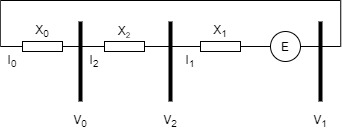
\includegraphics[width=8cm]{images/cc_1.jpg}
\caption{Circuito equivalente em componentes simétricas. Fonte: própria.}
\label{top4:fig:1} 
\end{center}
\end{figure}

Considerando o circuito da figura \ref{top4:fig:1}, observa-se que a corrente que circula pelas reatâncias de sequência positiva, negativa e zero são iguais. Como todas as reatâncias também são iguais, as correntes podem ser expressas por:

\begin{equation}
I_0 = I_1 = I_2 = \frac{E}{X_1+X_2+X_0} = \frac{E}{3X_1}  
\end{equation}
Considerando $E = 1 \, pu$, tem-se que cada uma das tensões em componentes simétricas são:

\begin{equation}
V_1 = E - I_1X_1 = E - \frac{EX_1}{3X_1} = \frac{2}{3}E 
\end{equation}
\begin{equation}
V_2 = V_0 = - I_2X_2 = -\frac{EX_1}{3X_1} = -\frac{1}{3}E \\
\end{equation}
Agora para obter as tensões $V_b$ e $V_c$, realiza-se a transformação inversa do domínio das componentes simétricas para o sistema de coordenadas abc, com $\alpha = 1 \angle 120^{\circ} $.

Uma vez que foi demonstrado os valores obtidos, recorre-se ao MATLAB para o cálculo da equação matricial de forma mais prática.

\lstinputlisting[language=Matlab,style=mystyle]{exercicio_5.m}

\begin{equation} \label{top4:exe5:1}
 \begin{bmatrix} V_a \\ V_b \\ V_c  \end{bmatrix} \,=\, \begin{bmatrix} 
  1 & 1 & 1 \\ 
  1 & \alpha^2 & \alpha  \\
  1 & \alpha & \alpha^2 \\  
 \end{bmatrix}\, 
 \begin{bmatrix} V_0 \\ V_1 \\ V_2  \end{bmatrix} \,=\, 
 \begin{bmatrix} 0 \\ 1 \angle-120^{\circ} \\ 1 \angle120^{\circ} \end{bmatrix} \, p.u
\end{equation}
Assim observa-se que as tensões para as fases as demais fases se mantiveram as mesmas devido ao equilíbrio no sistema. Outra forma de observar a inexistência de sobretensão, toma-se $K=1$ aplicado à equação \ref{fst} do fator de sobretensão, assim obtendo um fator unitário.

\subsubsection*{Exemplo 6 - curto-circuito}

Agora será analisado o mesmo curto-circuito, porém para uma rede isolada devido a ligação delta em um transformador. O delta do transformador atua como um filtro da corrente de componente zero $I_0 = 0$. A figura \ref{top4:fig:2} ilustra o problema.

\begin{figure}[H]
\begin{center}
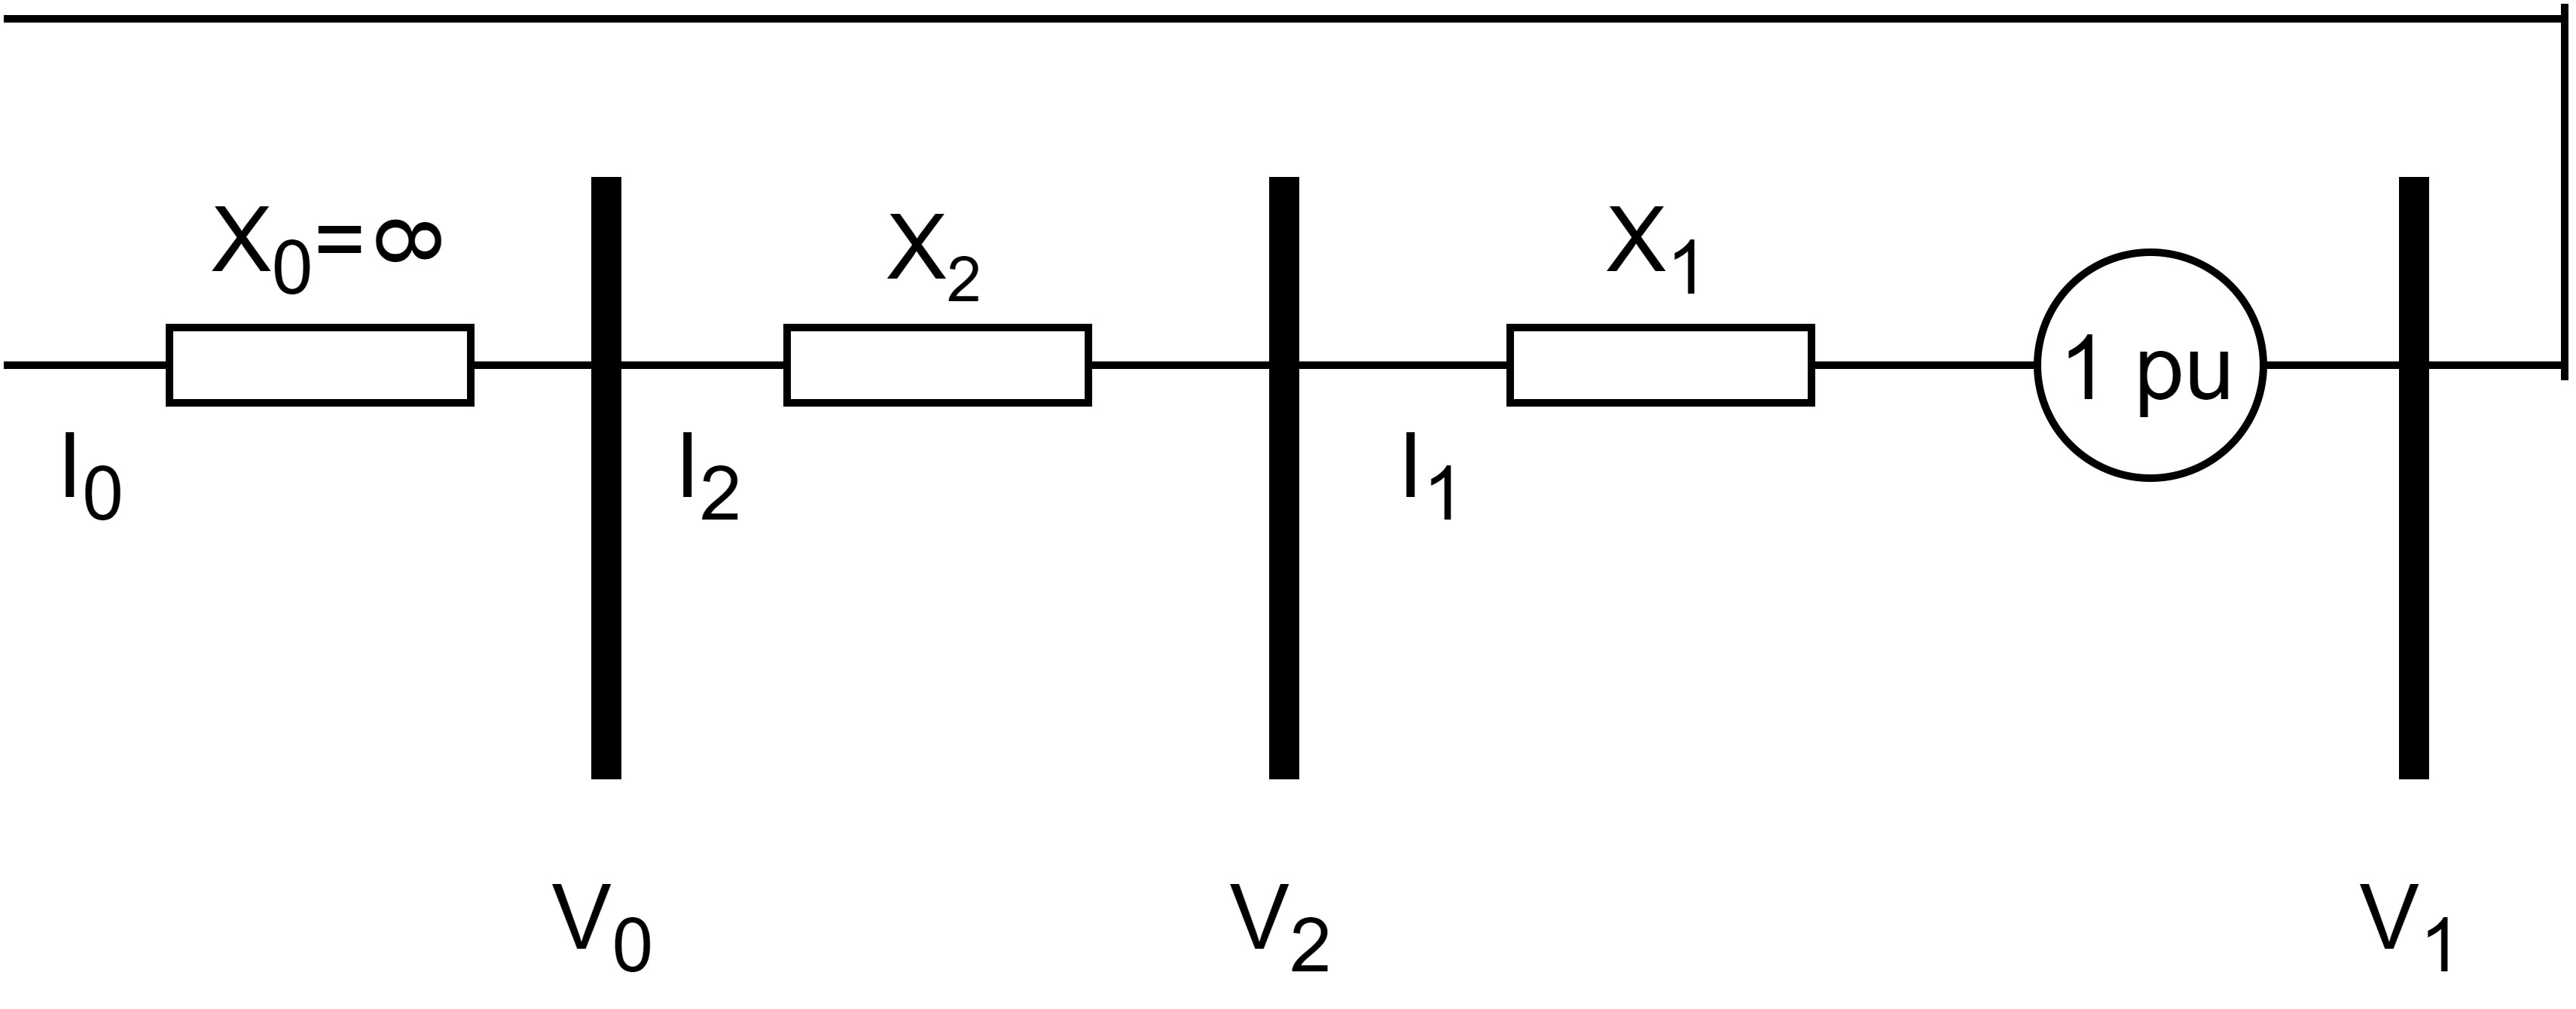
\includegraphics[width=8cm]{images/cc_2.jpg}
\caption{Circuito equivalente em componentes simétricas para uma rede isolada. Fonte: própria.}
\label{top4:fig:2} 
\end{center}
\end{figure}
Em decorrência da ligação série do diagrama de componentes simétricas, todas as correntes serão nulas devido a isolação: $I_1=I_2=I_0=0$. A tensão $V_1 = E$ e como a tensão de componente zero está diretamente em contato com a de componente positiva, seu valor será $V_0=-E$. Assim, para as mesmas considerações de $E$ e $\alpha$ do exemplo anterior, pela equação matricial \ref{top4:exe5:1} e a adaptação do código em MATLAB, encontra-se as tensões de componentes de fase:

\lstinputlisting[language=Matlab,style=mystyle]{exercicio_6.m}
\begin{equation} \label{top4:exe6:1}
 \begin{bmatrix} V_a \\ V_b \\ V_c  \end{bmatrix} \,=\, 
 \begin{bmatrix} 0 \\ 1.7321 \angle-150^{\circ} \\ 1.7321 \angle150^{\circ} \end{bmatrix} \, p.u
\end{equation}
Em termos de fator de sobretensão, considera-se $K=\infty$, pois $X_0/X_1=\infty$. Logo a parcela $\frac{\sqrt{K^2+K+1}}{2+K} = \frac{\sqrt{1 + 1/K + 1/K^2}}{1+2/K}$ do fator de sobretensão tende à unidade, implicando em $f_{st} = \sqrt{3}$.

\subsubsection*{Exemplo 7 - curto-circuito}

Este exemplo considera um curto-circuito fase-terra no fim da linha, alimentada em 525 kV ($V_L$), e solicita o cálculo das tensões nas fases não defeituosas. O circuito $\pi$ equivalente pode ser considerado o de uma linha longa de 300 km ($l$). A tensão do gerador $E$ será o equivalente da tensão nominal por fase; $X$ representa a reatância de linha; e $2X_c$ representa a reatância capacitiva da linha em cada uma das extremidades para os capacitores $C/2$. Seus valores serão:
\begin{center}
    $X_1 = X_2 = j90 \Omega; \, X_{c1} = X_{c2} = -j1473.6 \Omega$ \\ \vspace{1pt}
    $X_0 = j420 \Omega; \, X_{c0} = -j2210.4 \Omega$
\end{center}
Dessarte, para solucionar o problema é necessário retornar às equações impostas pela situação do exemplo 5 e generaliza-l-as para o caso da capacitância. Porém para a linha em aberto se faz necessário utilizar o equivalente de Thévenin para o caso genérico $X_y // 2X_{cy}$ (lembrando que o fator multiplicativo dois é oriundo de C/2). Assim, para cada uma das componentes simétricas, o equivalente de Thévenin será: $Z_{eq1} =  Z_{eq2} = j92.83\Omega$ e $Z_{eq0} = j464.09 \Omega$. Consequentemente, a tensão utilizada será a de vazio, que será a resultante sobre a parcela capacitiva da reatância, resultando no divisor de tensão: $E_v = \frac{2X_{c1}}{X_1+2X_{c1}} E = 1.0315E$. A tensão em vazio só é calculada para o circuito de sequência positiva, uma vez que apenas ele representa as fontes.

Retornando para as equações generalizadas das correntes e tensões, tem-se:

\begin{equation}
I = I_0 = I_1 = I_2 = \frac{E_v}{2Z_{eq1}+Z_{eq0}}    
\end{equation}
\begin{equation}
V_1 = E_v - IZ_{eq1} 
\end{equation}
\begin{equation}
V_2 = - IZ_{eq2} 
\end{equation}
\begin{equation}
V_0 = - IZ_{eq0} 
\end{equation}

Do código em MATLAB, as tensões em componentes simétricas e as tensões convertidas para componentes de fase serão:

\lstinputlisting[language=Matlab,style=mystyle]{exercicio_7.m}

\begin{lstlisting}[language=Matlab,style=consolestyle]
>> I = -0.481e3i; V1 = 267.99e3; V2 = -44.67e3; V0 = -223.21e3; Va = 0; abs(Vb) = abs(Vc) = 430.72e3; angle(Vb) = - angle(Vc) = -141.05.
\end{lstlisting}

Isso demonstra uma corrente de componente simétrica da ordem de $0.5 kA$, com tensões bem variadas ($V_1 = 267.99 kV$, $V_2 = -44.67 kV$ e $V_0 = -223.21 kV$). Quando transformadas para as componentes de fase nota-se a tensão da fase em curto realmente é nula $V_a=0$ e as demais são conjugadas entre si: $V_b = V_c^* = 430.72 \angle -141.05^{\circ}$.

O fator de sobretensão deve ser calculado para um $K = X_0/X_1 = 4.667$, resultando em $f_{st} = 1.3611$. Se considerar a capacitância, e $K$ a partir das impedâncias de Thévenin, ter-se-á $K = 5$ e $f_{st} = 1.3776$ que no caso também pode ser encontrado por $E_v/|V_b|$, ou seja, aumentando a sobretensão.


\newpage